%=========================================================================
% (c) Michal Bidlo, Bohuslav Křena, 2008

\chapter{Introduction}

The main goal of the project is to design and develop a mechanism for analyzing and notifying users about interesting changes in new uploaded submissions. Submission is a representation of results of tests series in ResultCloud. ResultCloud is a system for management of long-term testing results. The mechanism must support a few types of notifications (for example notifications by email or by twitter) and has possibility to add more. The analysis mechanism must also have interface for presentation results. An interested people would be able to get notifications about interesting results of the analysis.
% It is important and useful because the biggest part of the test results are not interesting and has useless information, like the same testing results. Thus, the main goal of the analyzing is to find the interesting results and show them to user.

Analyzing of submissions is very important because a lot of results are useless, in most cases they are the same data, so it doesn't give any important information. Analyzing helps to save developer's time, it finds useful information and notifies developers or other users about that and thus anyone at any time can easily find needed information, or to see statistics of project.

In the first part of the work I must learn inner architecture of ResultCloud. How it works. This help me to use better all the opportunities in design and programming that mechanism.

Next chapters describe (\textbf{Introduction in ResultCloud\ \ref{ch:resultcloud}}) ResultCloud system how it works and why it useful for developers, what is submission in ResultCloud, (\textbf{Analyzer Mechanism Design\ \ref{ch:analyzer_proposal}}) analyzer mechanism proposal and (\textbf{Analyzer Mechanism Imple\-me\-nta\-tion\ \ref{ch:analyzer_implement}}) implementation, (\textbf{Notification design\ \ref{ch:notification_proposal}}) notifications, why it is important, proposal and (\textbf{Notification mechanism implementation\ \ref{ch:notification_implement}}) implementation notification mechanism and (\textbf{Conclusion\ \ref{ch:conclusion}}) conclusion about all done work.

\chapter{Introduction in ResultCloud}
\label{ch:resultcloud}

This chapter will describe what is software tests, how ResultCloud works, why it is useful and all important moments for this bachelor's work, like what is submissions and how import of new series of tests results work.

\section{Testing}

Tests are one of the important part of software developing. Tests helps to developers find errors and fais in software. Many softwares has long developing proccess, this softwares demand an extensive series of tests. Series of tests is a file of test cases, it must test application or part of application.

Filip Matys in his bachelor's work use tool SystemTap for describe long-term tests. SystemTap has his own scripting language \emph{stap}. SystemTap use for test Linux kernel. SystemTap's series of tests is executed by tests interface DejaGnu. Series of tests can be consists more than one scripting files. SystemTap after running series of tests write output to text file.  

\section{What is ResultCloud}

As I wrote in introduction, ResultCloud is a system for management of long-term testing results. This means that ResultCloud collects testing results of some project, build diagrams based on that results, compare it, so developer can comfortably look at results or easily find the difference between them. Currently, there do not exist new, modern instruments for the presentation of tested results in readable form, because all instruments that we have now is too old, and does not extendable, as written by Filip Matys in his bachelor's work: “Tools which solve that problem [3], are too old and fall behind all modern applications. One of the biggest problem of that tools is no opportunity to expand and with growing market of different mobile devices with internet connection not able to present data in responsive form.” \cite{filip}. ResultCloud has more advantage, for example in ResultCloud parsing and management doing by plugins. Plugin is a plug-in module, that can be connected to ResultCloud in any time. Each plugin is written for one type of testing results. For example plugin “DejaGnu summary v1.0” can parse and show only SystemTap results. Thus ResultCloud is extendable system.

ResultCloud is useful for developing applications because it provides tools for present, compare and work with long-term test's results. For developers it is quite hard to look up for some information in a data bunch. But with ResultCloud developer only need to import results of tests series into ResultCloud, ResultCloud stores it and then presents it in a comfortable, readable form. For example: kernel of operation system need a lot of tests that collect into series of tests and for developer every time look for some interesting results take a lot of time, but ResultCloud store results in submissions, and then presents it like diagrams and lists of results, also provides some extendet tools for search interesting results, compares two or more submissions, thus developer can easily find or look at the results.

\subsection{Internal structure}

ResultCloud is a complex system. ResultCloud consists of two parts; frontend and backend. Frontend is a part on the client side, built with using of AngularJS. AngularJS is a JavaScript MVC (Model-View-Controller) framework which provides tools for build and work with web pages. In official documentation write next: "It lets you use HTML as your template language and lets you extend HTML's syntax to express your application's components clearly and succinctly. Angular's data binding and dependency injection eliminate much of the code you would otherwise have to write. And it all happens within the browser, making it an ideal partner with any server technology"\cite{angularJS}. Angular asynchronous connect with backend part. 

\subsubsection{Frontend (AngularJS)}

\begin{wrapfigure}{r}{0.5\textwidth}
  \centering
    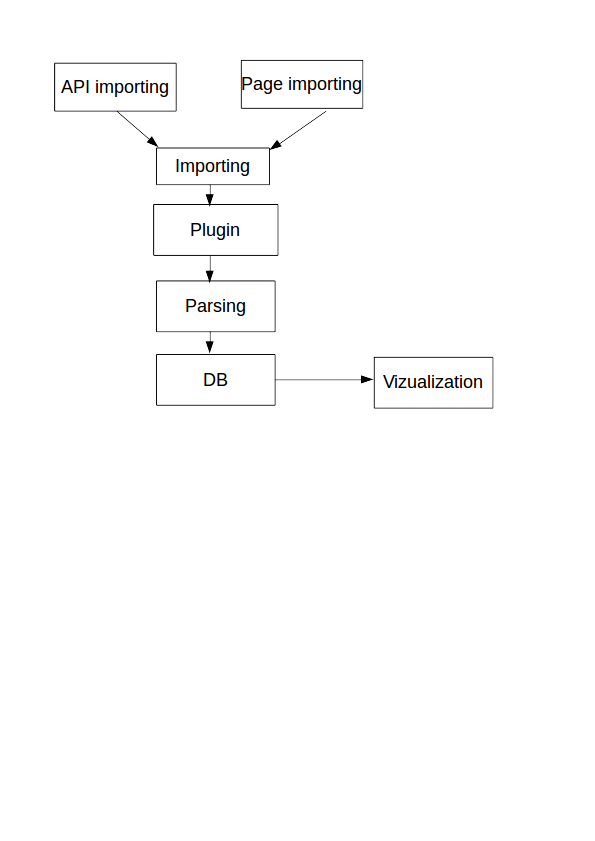
\includegraphics[trim=0 13.41cm 0 0,scale=0.5]{fig/result-cloud.png}
  \caption{ResultCloud architecture}
  \label{fig:result_cloud}
\end{wrapfigure}

For control whole page AngularJS uses controllers. Controller in Angular is defined by a JavaScript constructor function that used to increase Angular scope. Every controller has his own template, Angular automatically builds pages with template, according to data getting from controller's variable \emph{scope}. Controller has variable \emph{scope} that contains data for build page. AngularJS also has directives. Directives extend functionality of static HTML elements. A custom directive replaces the element for which it is actived by his own template. Thus it is easy to build complicated web pages that consists of more than one elements, and include external elements from other projects.

In ResultCloud, pages like login page, dashboard, project, plugin overview page and etc. use controller, but for build content use directives. Elements like submissions list, submission overview list and etc. using directives, it helps build more complicated pages, for example submission overview page use several directives, one for building list with results, one for building diagrams. 

\subsubsection{Backend}

Backend is also divideed on the smaller part. Controllers are on the top of hierarchy. This hierarchy can be seen in image\ \ref{fig:result_cloud}. Angular connect directly with controllers. Controllers are PHP classes. Controllers has only one mission, to get request and parsed data and give it to Services. Services are very important part, they get data and use different database entities, other services, plugins for returning result to the controller, which returns it to client.

For connecting with database there is exists a \texttt{DatabaseDriver} that connected to database, and use data access object (DAO). DAO contains all basic methods for work with database. Every entity must have DAO, which inherit basic DAO, and then system will work with entity through entity's DAO. Results of SELECT query converting to TSE (Test-Suite-Entity) object. TSE object helps to work easier with entities.


\subsection{Components}

All ResultCloud capabilities like submission overview, project overview and etc. are components, it means that they have their own settings and should be installed manually. Each component has his own configuration file in which defined component's ID, which plugins component support and other. Component system make possible to easily extend ResultCloud. But components can not save data or change it, components only prepare and vizualize data. Every component has his own frontend and backend part. Backend part is a file \emph{CBuilder} with \texttt{CBuilder} class, method \emph{Get} prepare data and return them. Frontend is a directive that get prepared data and vizualize them.   

\subsection{Utilities}

ResultCloud has utilities, the most important utilities that was used in this bachelor's work, are described here:

\textbf{LINQ} -- idea of this utility was gotten from C\# and rewritten to PHP. \texttt{LINQ} is a class for simplest working with arrays, it has a lot of methods for getting array elements, filtering array elements and doing other operations with arrays that can not do default PHP functions. In application \texttt{LINQ} wrap standard array, thus make complicated operations more readable.  

\textbf{ValidationResult} -- this tool was created for data validation, it wrap validate object and enable to validate it. Many methods in ResultCloud using \texttt{ValidationResult}. \texttt{ValidationResult} has attribute \emph{Data} which contain validate data, attribute \emph{IsValid} which contain validation state and attribute \emph{Errors} which contain array of strings that describe occurred errors.

\subsection{Data store organization}

Data organization in ResultCloud is represented in Plugins. Plugin parse and save specific formated test's results. In the past plugins has all demanded for self-installation, parsing and vizualization data, now vizualization is shared. 
Each plugin has own implementation of Parser to parse input data, and save it in a Project, Submission, etc. Submissions of the same software are grouped to \textbf{Project}. In submission, data orginized to \textbf{categories}. If file with tests results has no categories, ResultCloud create "Default" category. Categories are also divided to \textbf{TestCases}. TestCases contain \textbf{Results}.

In this bachelor's work I will analyse Submissions, their Results, and other stuff that may be interesting for people.

\section{What is Submission}

As I wrote earlier, the submission is a results of single series of tests. The smallest part of every submission is Result. This part contains result of a single test from series of tests. All other parts like Categories, TestCases are only organization unit. 

There are two ways to import a new Submission: first is through the web page, second is using an API. For import in first way need to sign in like a user in ResultCloud and go to import page, fill all fields and press import button, then Angular send request with file to \texttt{ImportController}. To import in second way need sign in through ResultCloud API and send file with other parameters by POST request to \texttt{import} class. 

Every plugin has a class \texttt{Parser}, for parsing files and putting them into Database (DB). When client send file to \texttt{ImportController} or to \texttt{import} class, it call \texttt{ImportService}, which find demanded plugin in DB, then include plugin's class \texttt{Parser} and call method \emph{ParseImport}. Parser returns to \texttt{ImportService} \texttt{SubmissionTSE} object, which contains all parsed data as TSE objects. \texttt{ImportService} than save it to DB and return successful result to Controller or API class.

\chapter{Analyzer Mechanism Design}
\label{ch:analyzer_proposal}

All analyzers must somehow unite into one working system. There must be a mechanism for that. Mechanism must not be complicated and easy for extend. Thus it must easy to control all analyzers and work with their results. This chapter will describe proposals on how impelement analysis mechanism better.

\section{Architecture} 

There are two types of architecture: module and built-in. Module type means that mechanism would be divided into modules, like “Divide and Conquer”, one of the main advantages is easy extending. Second type is built-in, which means that mechanism would be built-in into whole ResultCloud system, one of the main advantages of this type is working speed.

I choose first method, because difference in speed beetwen them would be to small, but easy extending advantage is that what mechanism demand. So let start from the main part, kernel of whole mechanism, \texttt{AnalyzerController}. 

\begin{wrapfigure}{r}{0.5\textwidth}
  \centering
    \includegraphics[scale=0.7]{fig/entity.png}
  \caption{Analyzer entity}
  \label{fig:entity}
\end{wrapfigure}

\section{AnalyzerController}

\texttt{AnalyzerController} would get all existed analyzers and use them. Mechanism also would provide entity for saving analysis data. Analyzer can not work with DB, because in practice it is normal to divide work between separated modules, thus analyzer only analyze input data and visualize it. Centralized method is good for that case because user don't need to load demanded analyzers and work with DB, all this operations do \texttt{AnalyzerController}.

\section{Analyzer entity}

In the picture presents entity \emph{Analyzer} \ref{fig:entity}, which contain four attributes. Attribute \emph{Submission} has ID of the submission, that analyzer results belongs to. \emph{Project} is alternative attribute to \emph{Submission}, it has ID of the project. \emph{Analyzer} contains machine analyzer ID. And \emph{Result} contains analyzer results, this is a text attribute, every analyzer has his own output results format.

\section{AnalyzerController structure}

\begin{figure}
  \centering
    \includegraphics[trim=0 22cm 0 0,scale=0.8]{fig/analyzer-struct.eps}
  \caption{Analyzer structure}
  \label{fig:an_struct}
\end{figure}

As can be seen in the image \ref{fig:an_struct}, \texttt{AnalyzerController} is center part of whole analyzer's mechanism. When application starts \texttt{AnalyzerController} finds all available analyzers, this is good for optimization. \texttt{AnalyzerController} is realize easy analyzer control. One method must run all analyzers that supports current submission's plugin, and returns result which \texttt{AnalyzerController} write to DB. Also \texttt{AnalyzerController} must consists methods for vizualizating data.

\section{Analyzers}

This section will describe design of Analyzers by itself and how it connected with analyzer controller.

\subsection{Analyzer design}

For correct connecting with analyzer controller, analyzer must has a static constant attribute with unique machine ID (under it ID, analyzer would be identified in Analyze entity), method for getting and processing data (name of the method must be the same for all Analyzer classes) and two methods for vizulizating data (Visualize, VisualizeSingle). Vizualizating methods will get data from \texttt{AnalyzerController} which get it from DB and return it in JSON format.

Method for process data gets in parameters: array of submissions, new submission and plugin name. It must returns \texttt{ValidationResult} object, with string in Data attribute, or array of strings if it has a few results, or it can returns empty result, with null in Data attribute.

Also analyzer has an attribute called \emph{is\_interesting} which contains status of previous analysis, and if analysis results is interesting it return true, in another case false, it need to notifying only about interesting submissions.

\begin{figure}
  \centering
    \includegraphics[scale=0.6]{fig/warframe.png}
  \caption{Template}
  \label{fig:temp}
\end{figure}

\subsection{Analyzer vizualisation}

Every submission has his own analysis results, those results would be presented in personal page. Image\ \ref{fig:temp} show that every analyzer has some space on that page. Because different analyzers use different methods for vizualization, there is need to specificate different possibilites to vizualize information. As mentioned in chapter \ref{ch:resultcloud} ResultCloud uses AngularJS for vizualize data and templates, so every analyzer must have his own template and AngularJS  directive. Image shows layout of analysis results.

\subsection{Kinds of Analyzer}

Next step is propose some kind's of analyzers. Here are analyzers whose results would be interesting for programmers.
\begin{itemize} 
\item \emph{Find strange changes like if result has a long time the same value and than it change}, it would be interesting because a lot of test cases has long time same result, so most of time it is just useless information, but changes is interesting and useful for developer.
\item \emph{Check a changes in tests, like if some test which is contained in all previous submissions dissapear}, it would be interesting and useful because changes in test cases by itself.
\item \emph{Check if some test had a long sequence of some bad value like FAIL or ERROR and then take a PASS, but after take FAIL or ERROR again}, it would be interesing because using this information can help developer to find why test always failing.
\item \emph{Check changes from UNTESTED to some result}, it would be interesting because unused test case started to be in use.
\item \emph{Check if presented a new tests}, it would be interesing because new tests can bring new useful information.
\item \emph{Check GOOD, BAD, STRANGE changes in tests}, it would be interesting because all changes can bring new useful information about program work. 
\item \emph{Check if count of bad results is get maximum}, it would be interesting because it notify developer about that changes caused a lot of bad results.
\end{itemize}

\chapter{Analyzer Mechanism Implementation}
\label{ch:analyzer_implement}

This chapter will describe mechanism's implementation. Mechanism implemented in PHP and JavaScript, because that languages was used for implementation ResultCloud. Mechanism would be implemented according to proposals in previous chapter.

\section{Structure}

Because analyzers are not plugins or any other components in ResultCloud, analyzers will be \emph{extentions}. Whole system has own directory \emph{analyzing}. Which contain one directory for analyzers - \emph{analyzers}, and one for templates - \emph{templates}. Root directory also contain \texttt{AnalyzeController}.

Analyzing starts only after new submission would be inserted into DB, in \texttt{ImportService} class.

\section{Entity}

\emph{Analyzer} entity was converted into ResultCloud acceptable format. As a result, three classes were created: \texttt{AnalyzerDao}, \texttt{AnalyzerTSE}, \texttt{AnalyzerService} and edited table installation class. \texttt{AnalyzerDao} class for work with \emph{Analyzer} table. \texttt{AnalyzerTSE} class is for easily work with \texttt{AnalyzerDao} returned data. \texttt{AnalyzerService} class is for different and more complicated operations with data.

\section{Analyzing}

\begin{figure}
  \centering
    \includegraphics[scale=0.8]{fig/analyzer-implementation.png}
  \caption{Analyzer implementation}
  \label{fig:an_impl}
\end{figure}

\subsection{AnalyzeController}

\texttt{AnalyzeController} is a kernel of whole analyze mechanism. \texttt{AnalyzeController} is implemented like static class (but PHP does not support static classes, thus all methods are static), because creates more than one class object unnecessarily. Image\ \ref{fig:an_impl} describe good how whole mechanism is implemented. \texttt{AnalyzerController} connect with analyzers, and through \texttt{AnalyzeService} writes data to DB and get it from DB.

When \texttt{AnalyzeController} be included, it executes \emph{InitAnalyzers} method, that scan \emph{analyzers} folder, puts all available analyzers together and save it to \emph{\textdollar{AnalyzerList}} attribute. Method \emph{GetAnalyzersList} will return \texttt{LINQ} object with \emph{\textdollar{AnalyzerList}}.

\emph{analyze} method gets all analyzers from \emph{\textdollar{AnalyzerList}}, and call it analyzer method. Then returned value, or values it write to DB, and check if results are interesting by getting boolean value from analyzer method \emph{isInteresting}, if results are interesting it add analyzer ID to \emph{\textdollar{interesting\_analyzers}} array. Analyzers ID which has interesting value can get by method \emph{GetInterestingAnalyzers}. Method \emph{analyze} get parameters: currently uploaded submission - \emph{\textdollar{submission}}, \texttt{LINQ} object with older submissions - \emph{\textdollar{submissionList}} and plugin name - \emph{\textdollar{plugin}}. Returning \texttt{ValidationResult} object with the analysis status.

\subsection{Analyzer1}

\texttt{Analyzer1} is a simple analyzer created like example of analyzer structure. Analyzer gets new submission and the last one, compare them, if they have differences, analyze results become interesting. There are three categories of changes: GOOD, BAD, STRANGE. Output result format is JSON. It supports only "systemtap" plugin.

Each analyzer must has method \emph{analyze}, which analyzing input submissions according to plugin name. Parameters are the same as has method \emph{analyze} in \texttt{AnalyzeController}. Output results are in format JSON, it uses JSON because of it simplicity. Attribute \emph{\$is\_interesting} is boolean type, and became \emph{true} only if analysis results are interesting, otherwise it is false. As mentioned in previous part, analyzer has method \emph{isInteresting}, which return value of \emph{\$is\_interesting} attribute.

\emph{ANALYZER\_ID} is constant attribute, that contains unique analyzer ID, that ID is used in \emph{Analyzer} table, like analyzer identifier. \emph{JS\_CONTROLLER} is also constant attribute which contains name of JavaScript file with AngularJS directive, it is used for vizualization analyzing results.

\texttt{Analyzer1} get last imported submission and new imported submission, than by using \emph{foreach} construction get each category from last imported submission (let call it \emph{category1}) and try to find category with the same name in new imported submission (let call it \emph{category2}), if the same category not exists it get next category, othewise it doing the same with test cases, it get each test case from \emph{category1} and try to find test case with the same name in \emph{category2}, if test cases with the same names was found, it compare their results, if results with the same key has different value and differnce is GOOD (FAIL $\rightarrow$ PASS), BAD (PASS $\rightarrow$ FAIL), STRANGE (FAIL $\rightarrow$ ERROR), it increment variable that responsible for one of the differnce types and in the end return \texttt{ValidationResult} object with result in JSON format. Example of result in JSON format:
\begin{alltt}
\{
    "Good": 8,
    "Bad": 3,
    "Strange": 0
\}
\end{alltt}

\subsection{Analyzer2}

\texttt{Analyzer2} is a sample analyzer, it looks for changes in submission's results, from UNTESTED to any other value. It has \emph{ANALYZER\_ID} - "analyzer2" and \emph{JS\_CONTROLLER} - "analyzer2.js". It support only "systemtap" plugin. Output result's format is JSON. It works in the same way like \texttt{Analyzer1}, it get last imported submission and compare it with new imported submission, if results with the same key have different value and last imported has value UNTESTED, analyzer save path to result and new value to object. Here is an example of that object in JSON format:
\begin{alltt}
\{
    "Categories": \{
        "systemtap.apps": \{
            ".\textbackslash{}systemtap.apps\textbackslash{}mysql.exp": \{
                "mysql sdt app": "PASS"
            \}
        \}
    \}
\}
\end{alltt}

\section{Vizualization}

As was mentioned in chapter \ref{ch:resultcloud} ResultCloud use AngularJS for vizualization data. AngularJS is JavaScript MVC (Model-View-Controller) framework, every page has own controller, thus analyzer page must has it too. \texttt{AnalyzeController.js} is a file that contains controller for analysis result page. \emph{analyze.html} is a page template. Some of the page, that contain several sort of data, builded with the simplest part \emph{Components}, each component has individual settings, and individual Angular \texttt{directory}. Each component has \texttt{backend}, \texttt{frontend} folder and configuration file \emph{config.xml} with all settings and supported plugins. Backend folder consists \texttt{CBuilder} class, which return prepared data for representation. 

\begin{figure}
  \centering
    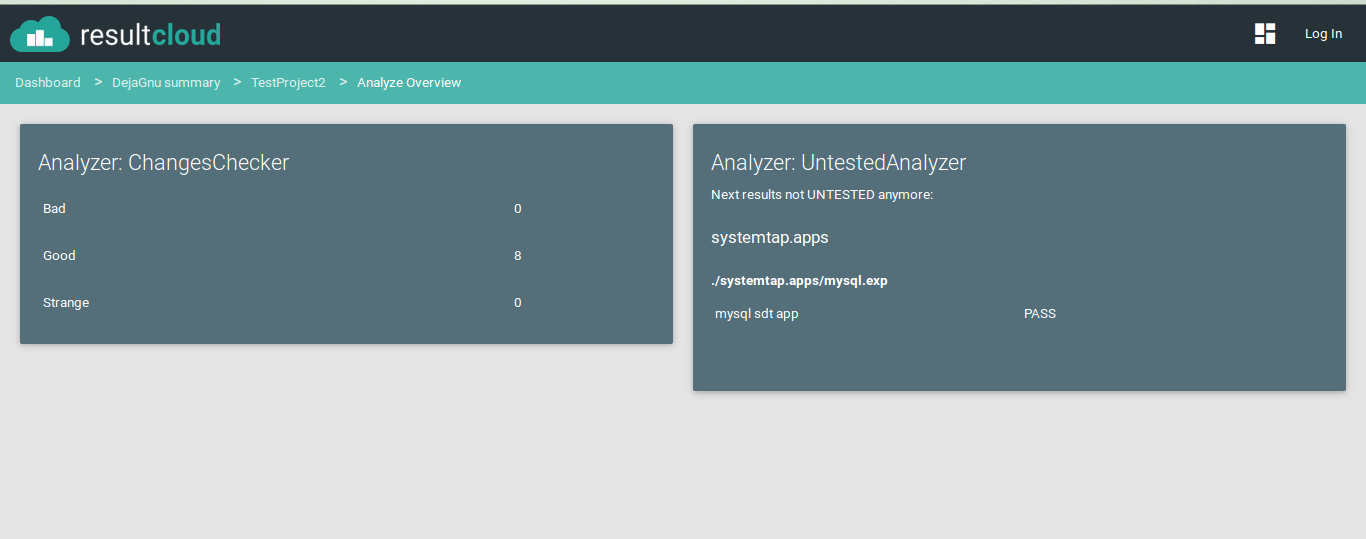
\includegraphics[scale=0.3]{fig/temp_res.png}
  \caption{Implemented template}
  \label{fig:temp_res}
\end{figure}

Analyzer page would use only one component \texttt{analyzeOverview}.It wouldn't have any settings, and will support all plugins. Angular directory firstly get array of analyzing results for current submission, than for each analyzer find own Angular directory, which put analyzer data to template and represent it. There some interesting part of code, how implemented inserting analyzers directive into \texttt{analyzeOverview} component template:
\begin{alltt}
$scope.buildAnalyzerView = function (key) \{
	\textbackslash\textbackslash Check if key not empty
    if (!$(key).length) \{
    	\textbackslash\textbackslash Make new scope clone from rootScope
        var data2 = $rootScope.$new();
        \textbackslash\textbackslash Include into cloned scope analyzer data
        data2.data = $scope.data[key];
        \textbackslash\textbackslash Compile analyzer directive tag with cloned scope
        var el = $compile('<' + key + '/>')(data2);
        \textbackslash\textbackslash Put result into page
        $("#"+key).append(el);
    \}
\}
\end{alltt}

Image\ref{fig:temp_res} present how it actually look. 

\texttt{CBuilder} class for \texttt{analyzeOverview} get \texttt{stdClass} object with attribute \emph{Submission} - submission ID. And call \texttt{AnalyzeController} method \emph{VisualizeBySubmission}. \emph{VisualizeBySubmission} get submission ID, for each analyzer get last inserted result, and give it to analyzer's method \emph{VisualizeSingle}, which parse results and return it like array. Then \emph{VisualizeBySubmission} puts vizualization data together into associative array the key analyzer ID and value analyze results, and return it.

\section{Evaluation}

During making bachelor's work was implemented analysis mechanism: \texttt{AnalyzerController} and two analyzers. All stuffs that was described in this chapter was implemented and functioning. Also mechanism are extendable, thus there is no problem to add new analyzers or new methods to it. Analysis results can be displayed in any format (list, diagram and etc.).

\chapter{Notification design}
\label{ch:notification_proposal}

Notification mechanism must be flexible, and easy to extend. This chapter contains proposals for implement notification mechanism. Here will consider mechanism's architectures, how implement notifiers better and notifications settings. 

\section{Architecture}

Like in case with Analyze Controller, I would divide notifications methods to the separated classes and Notification Controller will control them. But as opposite to analyzers there are several types of notifiers. First type is public notifiers, it means that notifications would be sended into some shared or public resources, like \emph{Twitter} for example. Private is means that it notifies each user separetly. According to this private notifiers must has settings, where user can set if he want to get notifications or not, and other options.

\section{Notification Controller}

Notification controller would has method for easy control notifications, which get all demanded fields, as \emph{title}, \emph{body}, \emph{bodyShort} (for resources that accept only short messages), \emph{adreses} (list of all adreses that must recieve notification) and according to them send notifications. Also \texttt{NotificationController} must provides methods for getting private and public \texttt{Notifiers}. When it included, it scans space for available \texttt{Notifiers}.

\section{Notification settings}

There must be a mechanism for adding settings to \texttt{Notifier} easy, and settings must be present at user's settings without editing any template for it. But user can edit only private settings, because public notifier settings are shared with other users, ResultCloud does not support user's hierarchy, thus nobody can edit public notifier settings.

ResultCloud provides good tools for work with settings, like entities \texttt{TemplateSettings} and \texttt{TemplateSettingsItem}. \texttt{TemplateSettings} is for saving setting's template information into DB, such as setting type, setting name and etc. \texttt{TemplateSettingsItem} is for save settings value.

\section{Notifier}

\texttt{Notifier} is a base part of notification mechanism, without at least one notifier it is useless. \texttt{Notifier} provides notification by itself, each notifier has own notification method, for example, by email, or Facebook.

\subsection{Notifiers architecture}

Every \texttt{Notifier} must have unique identifier(ID) for correct processing, by that ID \texttt{Notifica\-tion\-Controller} would identify notifiers, and it would have reference to notifier by this ID in settings template. \texttt{Notifier} must have one method for notification, and one method with settings. Each notifier has the same settings, thus that method can be picked out into some basic class, which would be inherited by notifiers classes. \texttt{Notifier} must have attribute that identifies it is like private or public notifier.

As a notify method in \texttt{NotificationController}, notify method in \texttt{Notifier} get the same parameters, except address, address is not associative array, but it is a simple array with addresses supported in that notifier. 

\subsection{Notifier types}

Within the confines of this bachelour's work, must be implemented these types of notifiers:
\begin{itemize} 
\item Email - notifications will be sent by email, this is private notifier
\item Twitter - notifications will be sent into prepared twitter account, public notifier
\item RSS - notifications will be present in RSS file, public notifier
\end{itemize}  

\chapter{Implementation of notification mechanism}
\label{ch:notification_implement}

This chapter contains description of notification mechanism implementation. As can be seen in image, \texttt{NotificationController} is a kernel, all notifiers are extended from \texttt{BaseNotifier} class.

\section{Structure}

Like analyzers, notification mechanism is not a plugin or any other ResultCloud kernel part, thus it also be in \emph{extentions} folder, in own \emph{notification} folder. \texttt{NotificationController} is also located in root directory. All notifiers are located in \emph{notifiers} folder.

Notification starts only if analyzer return interesting result.

\section{Settings}

Basically all notifers have same setting, this settings would enable or disable notifier's notifications. But as mentioned in previous chapter, only private notifiers can use settings. Notification mechanism does not work with settings, because list of addresses and notifiers must be assamble by those who send, notification mechanism only takes this list and send notification. 

ResultCloud has tools for settings, not only in server side, but also in client side it has automatic form generation for settings. Here is example of default \emph{getSettings} method in \texttt{BaseNotifier} class, to understand how set up settings better:

\begin{alltt}
public function getSettings()
\{
    \$settings = array();
    \$settingsItem = array();

    \textbackslash\textbackslash Setting label
    \$settingsItem['label'] = "Get notifications by this way";
    \textbackslash\textbackslash Setting ID for TemplateSettings entity
    \$settingsItem['identifier'] = "get-notify";
    \textbackslash\textbackslash Default value
    \$settingsItem['default'] = "1";
    \textbackslash\textbackslash Field type
    \$settingsItem['type'] = TemplateSettingsItemType::CHECKBOX;
    \textbackslash\textbackslash Is setting required
    \$settingsItem['required'] = 'true';
    \$settings[] = $settingsItem;

    return \S$settings; 
\}
\end{alltt}

\section{Notification}

\begin{figure}[hb]
  \centering
    \includegraphics[scale=0.6]{fig/notification_impl.png}
  \caption{Implementation of notification mechanism}
  \label{fig:not_impl}
\end{figure}

\subsection{NotificationController}

Like in case with \texttt{AnalyzerController}, \texttt{NotificationController} is static too, all methods are static, because there is no reason to create more than one class instance in application. Notification mechanism scheme\ref{fig:not_impl} showing how \texttt{NotificationController} connecting with other mechanism elements.

When \texttt{NotificationController} is included, it starts method \emph{preLoad}, this method scans \emph{notifiers} folder, include and assamble array with all available notifiers. There is exist a method for notifing \emph{notify(title, body, bodyShort, to)}, where \texttt{title} - is title of notification message, \texttt{body} - the longest body text, \texttt{bodyShort} - short body of the message but no longer than 140 letters, \texttt{to} - is an array of all adresses with the key of notifier ID. Method \emph{notify} calls notifier's function \emph{notify} only for notifiers which have their IDs in \texttt{to} parameter's key.

\texttt{NotificationController} also has different sorts of get's methods: \emph{getNotifyIds} (returns IDs of all notifiers), \emph{getPrivateNotifiers} (returns array with IDs only for private notifiers) and \emph{getNotifierById} (returns notifier object by notifier ID).

\subsection{Notifier}

Every notifier must inherit \texttt{BaseNotifier} class with default settings, and if it is need to define own method \emph{getSettings} that in the begining call \emph{parent} method. Also notifier must have unique ID in constant \emph{NOTIFY\_ID}. \emph{NOTIFIER\_PUBLIC} is constant, which contains boolean value, if notifier is public it contain \emph{true}, otherwise \emph{false}. The most important method is \emph{notify}, it has same parameters such as method \emph{notify} in \texttt{NotificationController}, except last address parameter, notifier would not get associative array, but gets a simple array with addresses.

\subsection{Notify1}

\texttt{Notify1} is a private notifier that send notifications by email. It gets array with email addresses and sends emails via default PHP \emph{mail} function. Here is notifier parameters:

\begin{alltt}
const NOTIFY_ID = "notify1";
const NOTIFIER_PUBLIC = false;
\end{alltt}

\subsection{Twitter}

\texttt{Twitter} is a public notifier that sends new twittes with some interesting information to twitter account. Now it connected to my account \href{https://twitter.com/cyberbond95}{cyberbond95} . If analyzer would have interesting results it sends new twitt to my account, and everyone can see it.

\texttt{Twitter} work with Twitter API by using \texttt{TwitterAPIExchange} library, which was suggested in Twitter API documentation \cite{twitter}. It has MIT license. Page of \texttt{TwitterAPIExchange} with examples \url{https://github.com/J7mbo/twitter-api-php}.

\subsection{RSS}

\texttt{RSS} is a public notifier that create or update \emph{rss.xml} file in root folder. \emph{rss.xml} presents one news for each project, if \texttt{RSS} get news for already existing in \emph{rss.xml} project, it updates news, otherwise it just create new one. Current actual version of RSS is 2.0, according to specification \cite{rss} second version is simplier than first.

\texttt{RSS} works with RSS by using \texttt{SimpleXML} that is default in most PHP versions. Here RSS example:
\begin{alltt}
<?xml version="1.0"?>
<rss version="2.0"> 
<channel>
<title>ResultCloud News</title>
<link>http://result-cloud.org/</link>
<description>ResultCloud analysing results</description>
<language>en-us</language>
<docs>http://result-cloud.org/rss.xml</docs>
<item>
<title>Project TestProject has new interesting submission</title>
<description>Submission with id 22 has interesting results according\\ to [analyzer1] analyzers, for more information go there\\ http://corly.local/#/project/1/analyze/22</description>
<link>http://corly.local/#/project/1/analyze/22</link></item>
</channel>
</rss>

\end{alltt}

\section{Evaluation}

Notification mechanism support adding new notifiers (if notifier was implemented like it was described in this chapter) and extending settings. \texttt{NotificationController} and three type of notifiers was implemented. One of notifiers is private email notifier. Other two notifiers are public.

During testing was found two problems: email sending on my computer get a lot of time, Twitter do not allow to send two twits with the same content. First problem is a local and related with software on my computer. Second problem is actual only when debuging, because in production content always will be different, in production current ID value for table never be discard, thus url in twit always be unique. 

\chapter{Conclusion}
\label{ch:conclusion}

In this bachelor work was proposed mechanism of analyzing tests results and notifing users about it, this mechanism must be easy to extend. There must be available more than one notifier for wider using.

Mechanism was built under ResultCloud system by using PHP and JavaScript (AngularJS framework). It consists of two parts: Analyzers and Notifications. Implemented kernel (\texttt{AnalyzerController}) and two analyzers in analyzer part. Implemented kernel as well (\texttt{NotificationController}) and three notifiers in notification part. And other parts was implemented for integrate mechanism into ResultCloud, like services for work with DB, different Angular directives for vizualization data.

Mechanism can be extending by adding new analyzers and notifiers. Also can be extending notification mechanism by adding new settings, for example: user can choose about which analyzers he wants get notification. Extend analyzer mechanism, add to each analyzer configuration file, and make it switchable like components in ResultCloud.

%=========================================================================
